\chapter{Experimental Results}

In this chapter I will present the experimental setup and results obtained during this thesis realization. Most of the results concern the characterization of the two cavities, their stabilization and their noise profile. Another important conclusion is the possibility of moving the cavity waists, enabling the dual color mode of BriXS. 

\section{Experimental setup}
\begin{figure}
	\centering
	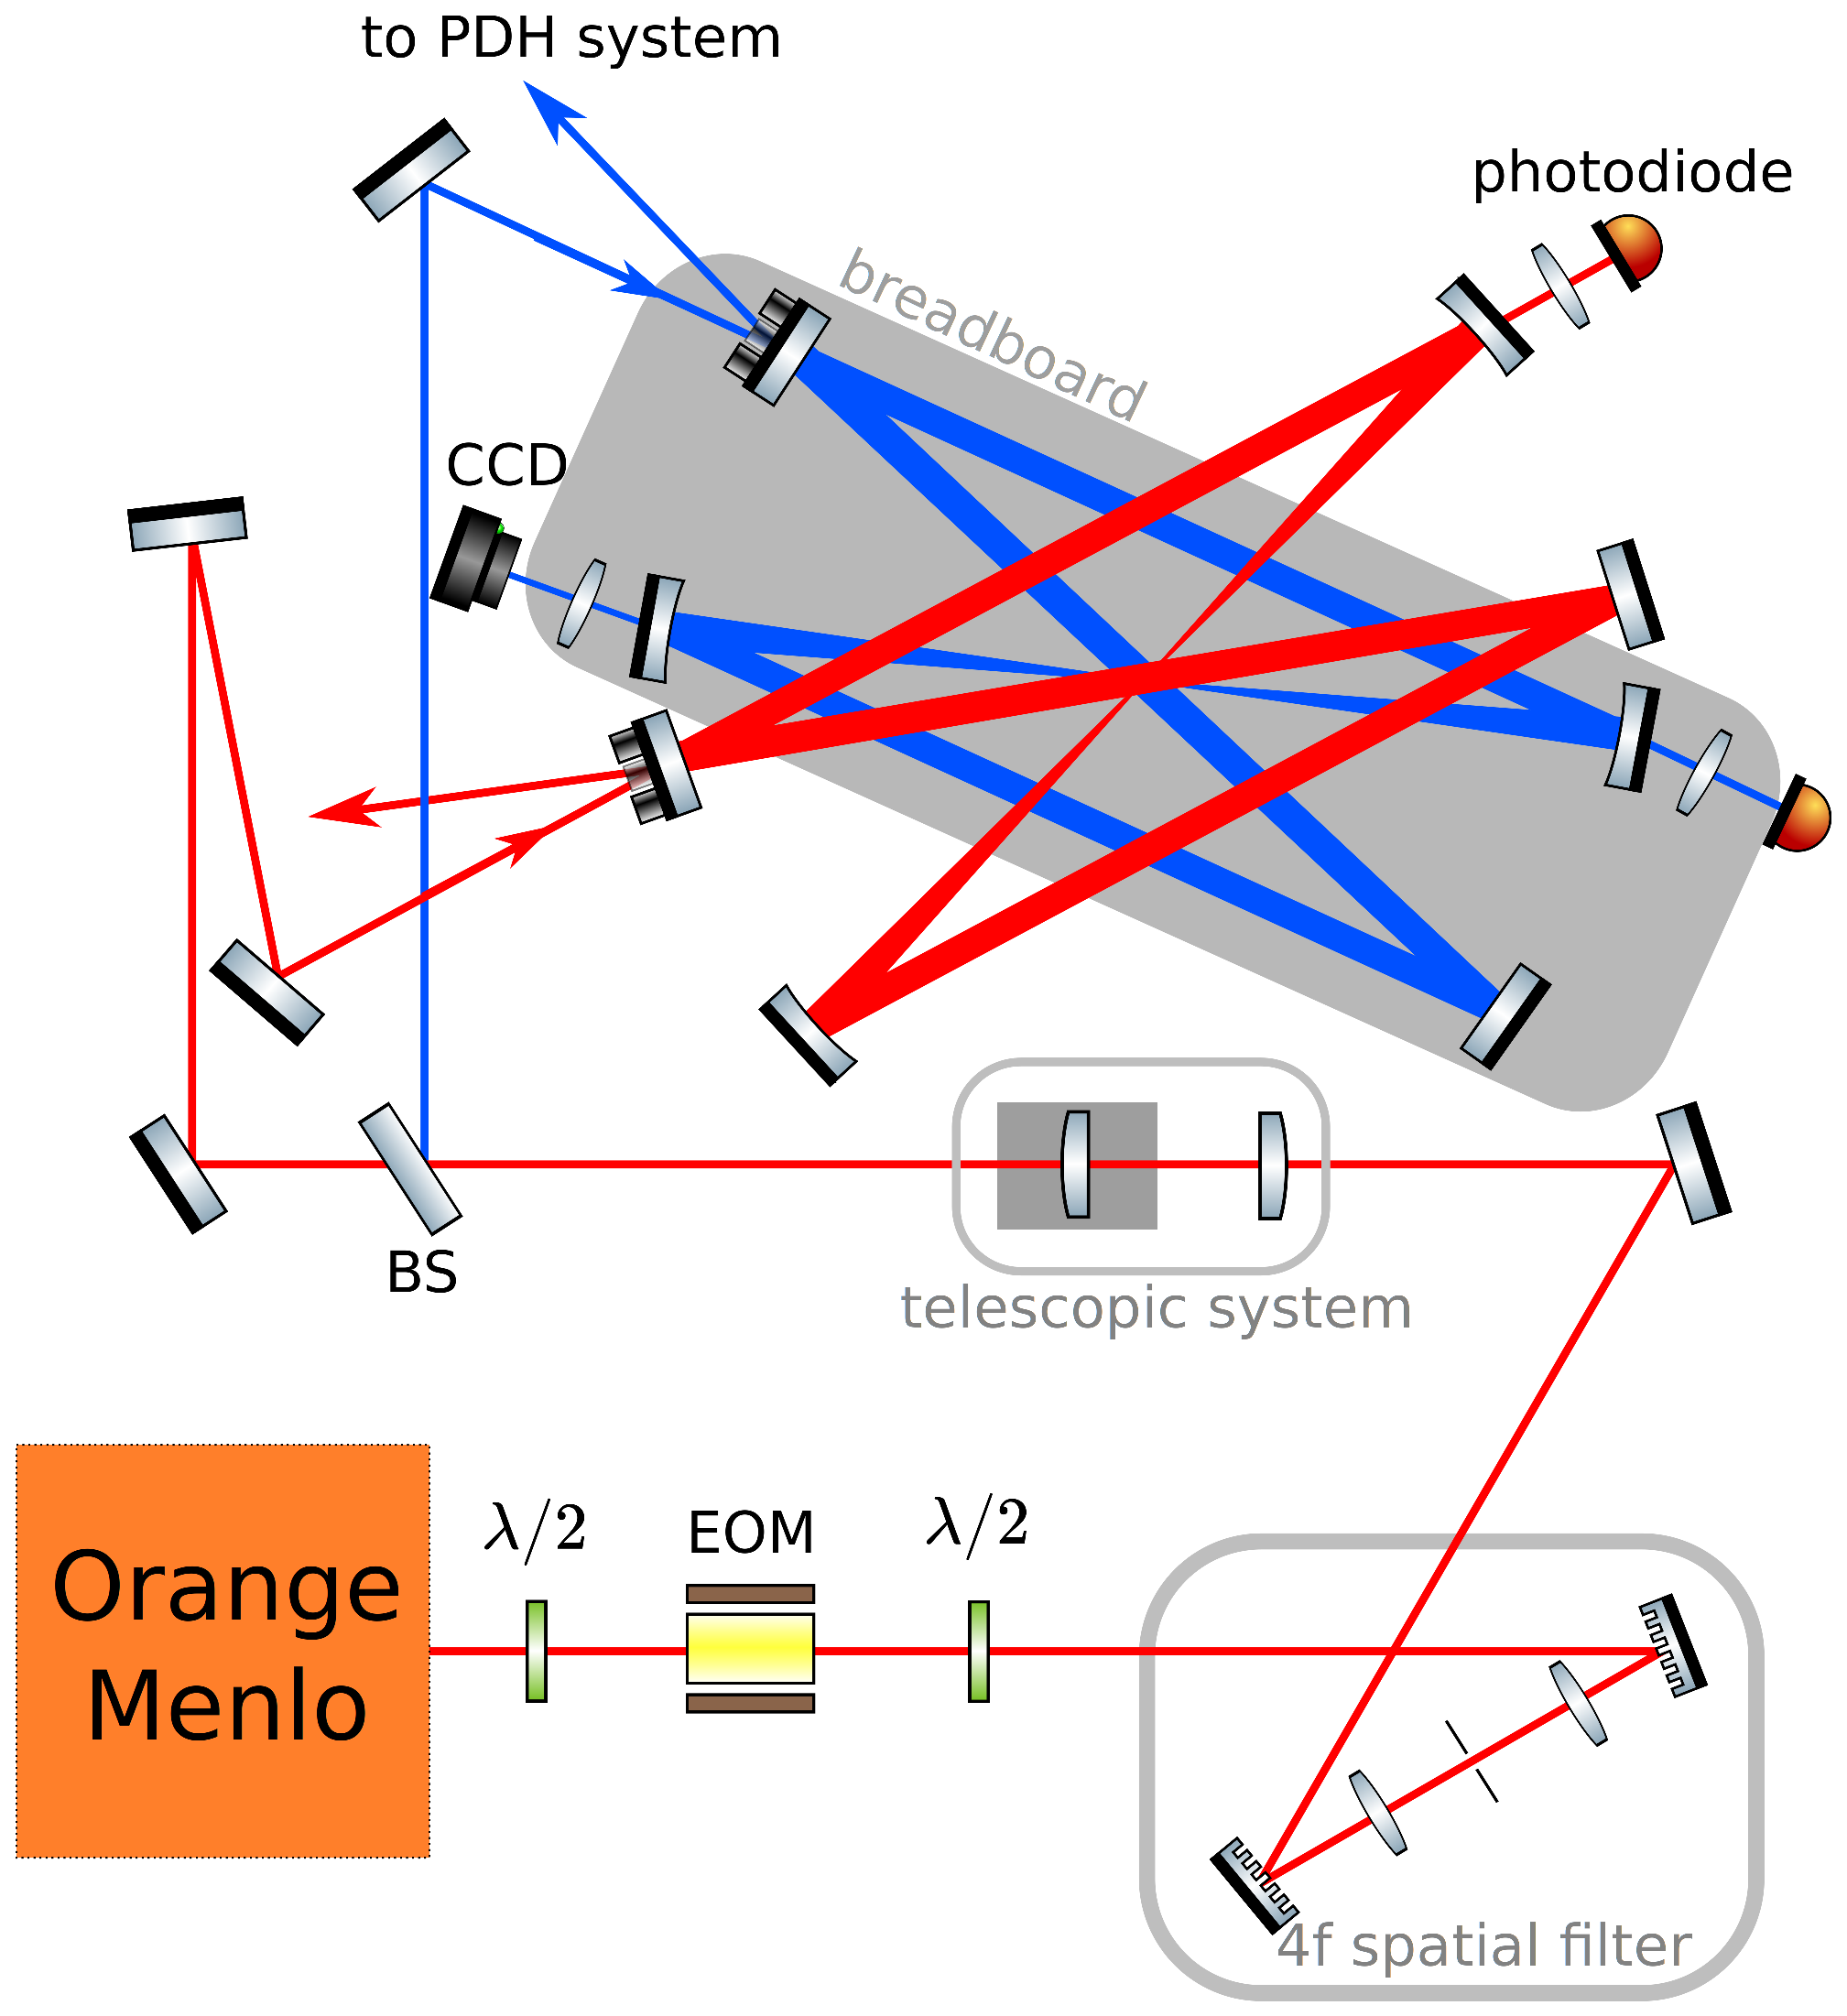
\includegraphics[width=1\linewidth]{images/schema.eps}
	\caption{The experimental setup. The 4f spatial filter consists in two diffraction gratings (1200 lines/mm) and two lenses ($f=100$\,mm), different frequencies focalize at different transverse positions and are selected by a slit between the lenses. The telescopic system can be adjusted by moving one of the lenses with a sled. Different colors are used only to highlight the two cavities. The transmitted beams are monitored with photodiodes and a CCD camera. The reflected beams are used by the two stabilization systems (see Fig \ref{fig:pdh}).}
	\label{fig:schema}
\end{figure}
\begin{figure}
	\centering
	\includegraphics[width=1\linewidth]{images/setup.jpg}
	\caption{The two crossed optical cavities realized in our laboratory.}
	\label{fig:setup}
\end{figure}
The Menlo Orange oscillator and the cavities are placed on an optical table covered with a laminar flow hood. The pulses exiting the laser source pass through an electro-optic modulator to generate two 3.5\,GHz sidebands around the carrier frequency, needed for the PDH system. Then it goes through a 4f spatial filter used to regulate the spectral width of the beam entering the cavities, a reduced spectrum improves the spectral coupling with the cavity but reduces the laser pulse power: a good compromise for the current cavities is a bandwidth with $\Delta\lambda = 3\,$nm.
The polarization is controlled with half-wave plates. A telescopic system with two lenses ($f_1 = f_2= 75$\,mm) is used to regulate the beam radius $w$ and its divergence to ensure maximum spatial coupling with the resonators. A beam splitter divides the pulse in order to seed both cavities.

\subsection{Bow-tie cavities}

Currently the two cavities are very different since the R\&D program proceeds step by step: the $\alpha = 7\degree$ cavity (from hereafter ``blue cavity'') is the more advanced one while the $\alpha = 30\degree$ cavity (the ``red cavity'') is a precedent prototype that was built in the program.

The blue cavity is composed of dielectric mirrors with high reflectivity\footnote{Ther mirrors are from Layertec company, the nominal reflectivity is $>0.99995$ for mirrors B C D, we later found the total reflectivity by measuring the mirror finesse and the coupling efficiency.}, the expected Finesse is about 770. The curved mirrors have a nominal radius of curvature of 750\,mm. The mirrors are mounted on a breadboard to reduce the mounting heights and to decouple the mirror oscillations from the optical table oscillations. The input coupler has a nominal reflectivity of 99.2\%, giving an expected enhancement factor of about 480; it is mounted on the piezo ring crystal used by the stabilization system. A piezo-controlled positioning system by SmarAct (Fig \ref{fig:smaract}) is used for aligning the cavity and finding the exact cavity length to satisfy the temporal condition, but also for the spot size compensation method and for moving the cavity waist.
\begin{figure}
	\centering
	\includegraphics[width=0.9\linewidth]{images/smaract.png}
	\caption{The SmarAct tilting mirror and the SmarAct positioning stage used for the alignment of the cavity and the moving of the beam waist.}
	\label{fig:smaract}
\end{figure}
To align the external beam with the cavity axis ray two mirrors outside the cavity are used, one of which is the beam splitter. The transmitted beams are used to monitor the power inside the cavity and for imaging purposes, while the reflected beam is used by the stabilization system.

The red cavity mirrors have lower reflectivities, giving a Finesse of about 410. The radius of curvature of the curved mirrors has been measured to be $R_B = 767$\,mm and $R_C = 741$\,mm.

The total cavity length is the same for both cavities and equal to 2990\,mm.

\subsection{The PDH stabilization systems}
\begin{figure}
	\centering
	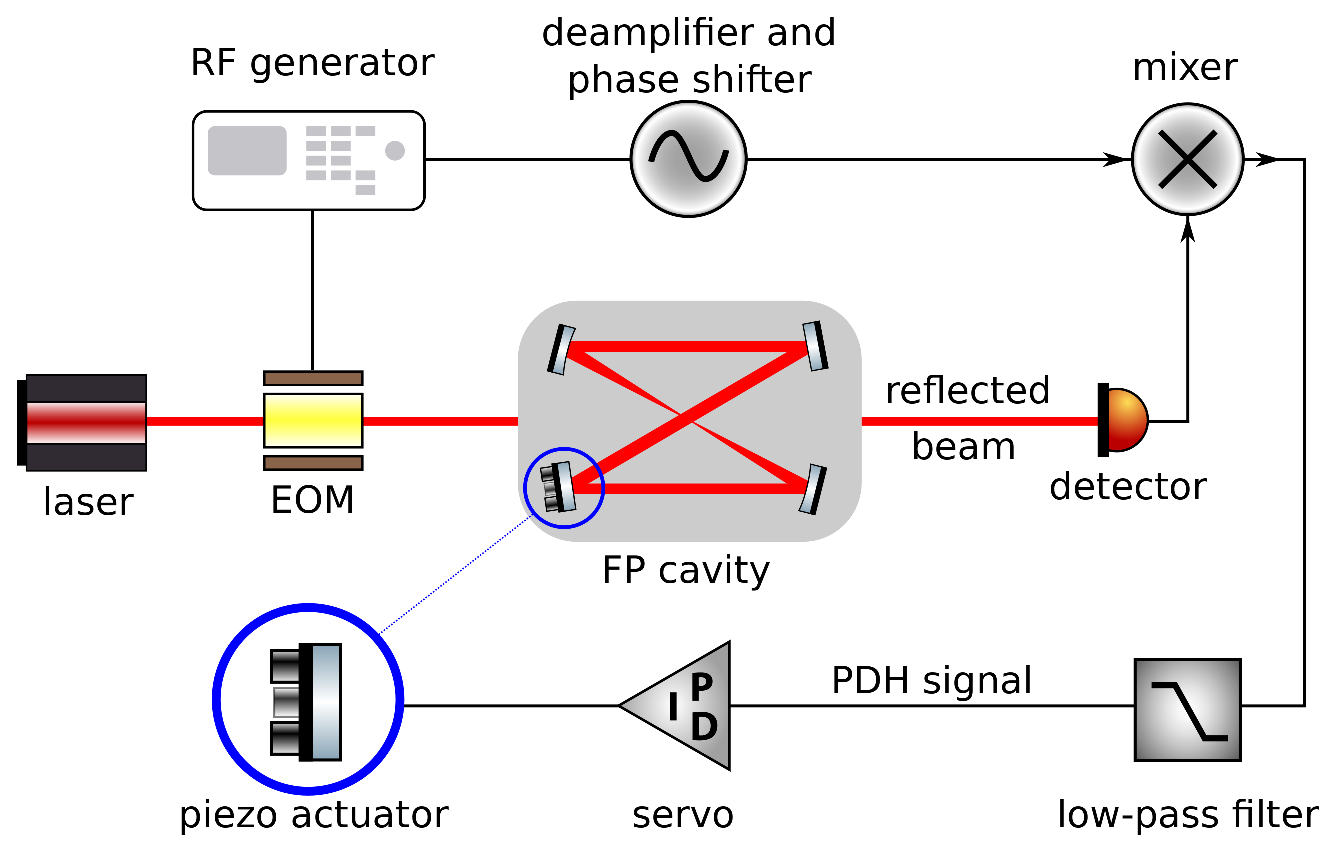
\includegraphics[width=1\linewidth]{images/pdh.eps}
	\caption{The PDH stabilization system scheme. The RF generator drives the EOM with a 3.5\,GHz sinusoidal wave to produce the sidebands. The reflected power signal (in which the sidebands and the carrier wave interfere) is demodulated with the same sinusoidal wave (controlled in phase and amplitude). After a pass through a 6th order Butterworth low-pass filter we have the PDH error signal (Fig \ref{fig:pdhtra}). The error signal is fed through a servo PID that then drives the actuator inside the cavity, adjusting the length and maintaining the stabilization with the external laser source.}
	\label{fig:pdh}
\end{figure}
The stabilization systems (one for each cavity) are composed by an electro optic modulator, a detector, a phase shifter, a mixer and a filter that togheter form the discriminator that produces the error signal. The signal is then fed to a servo PID\footnote{Only the integral and proportional stages are present in our system.} that drives the piezo actuator. The scheme is represented in Fig \ref{fig:pdh}.

\subsubsection{Stabilization procedure}

Here is the procedure we followed to stabilize the cavities and make them resonate:
\begin{enumerate}
	\item We align the cavity and the external mirrors by making sure the beam superimposes with itself after a round-trip.
	\item We send a triangular wave to the piezo to scan the cavity and we monitor the transmitted power searching for the resonance.
	\item We adjust the cavity length using the sleds until resonance is achieved, when this happens we see spikes in the transmitted power corresponding to different modes that resonate in the cavity (as in Fig \ref{fig:goodspa}).
	\item Using the external mirrors, the input coupler and the telescopic system we optimize the spatial coupling efficiency, maximizing the power coupled with the $HG_{00}$ mode and minimizing that coupled with other modes.
	\item We monitor the reflected power and the error signal and optimize its shape acting on the phase shifter (Fig \ref{fig:pdhtra}).
	\item We stop the scanning triangular wave and we search for the resonance by acting manually on the piezo voltage.
	\item Around resonance we activate the integral and the proportional stages to lock the cavity.
	\item The cavity is now stabilized, to optimize the parameters of the PID (integrator and proportional gain and the filter cut-off frequency) we look at the integrated spectral noise on the oscilloscope, minimizing it.
\end{enumerate}
\begin{figure}
	\centering
	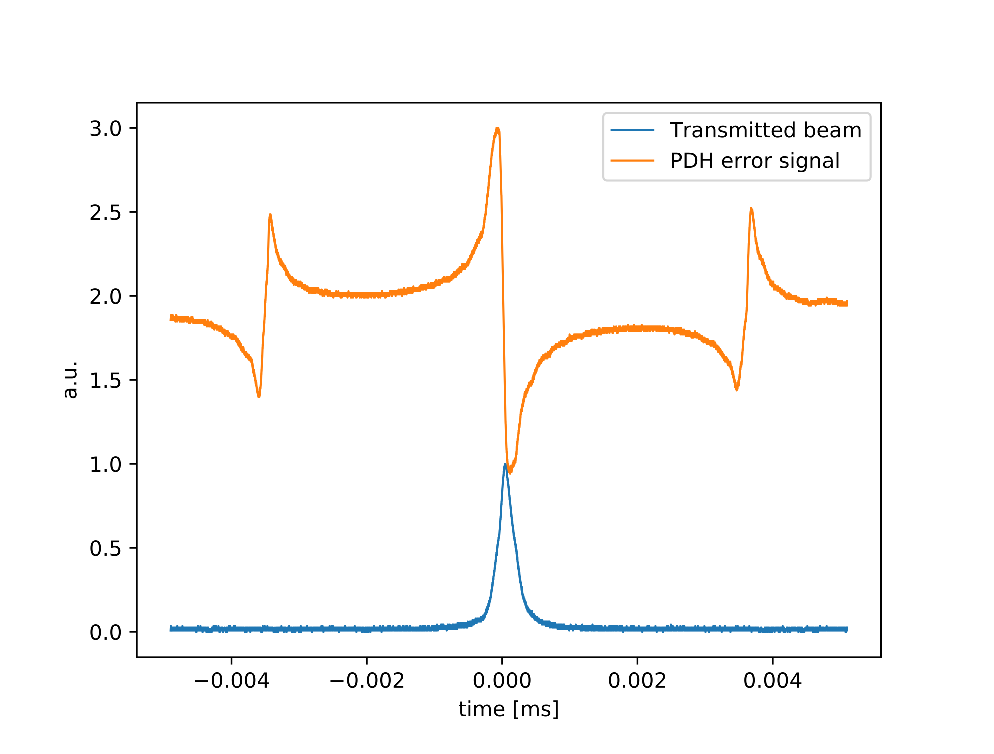
\includegraphics[width=1\linewidth]{images/pdhtra.eps}
	\caption{The PDH error signal produced by the discriminator during a cavity scan.}
	\label{fig:pdhtra}
\end{figure}
\begin{figure}
	\centering
	\includegraphics[width=0.5\linewidth]{images/foto/fotodiodo.jpg}
	\caption{The Thorlabs photodiode used to monitor the blue cavity transmitted beam.}
	\label{fig:fotofotodiodo}
\end{figure}

\section{Experimental measurements}

\subsection{Cavity Finesse measurement}
\begin{figure}
	\centering
	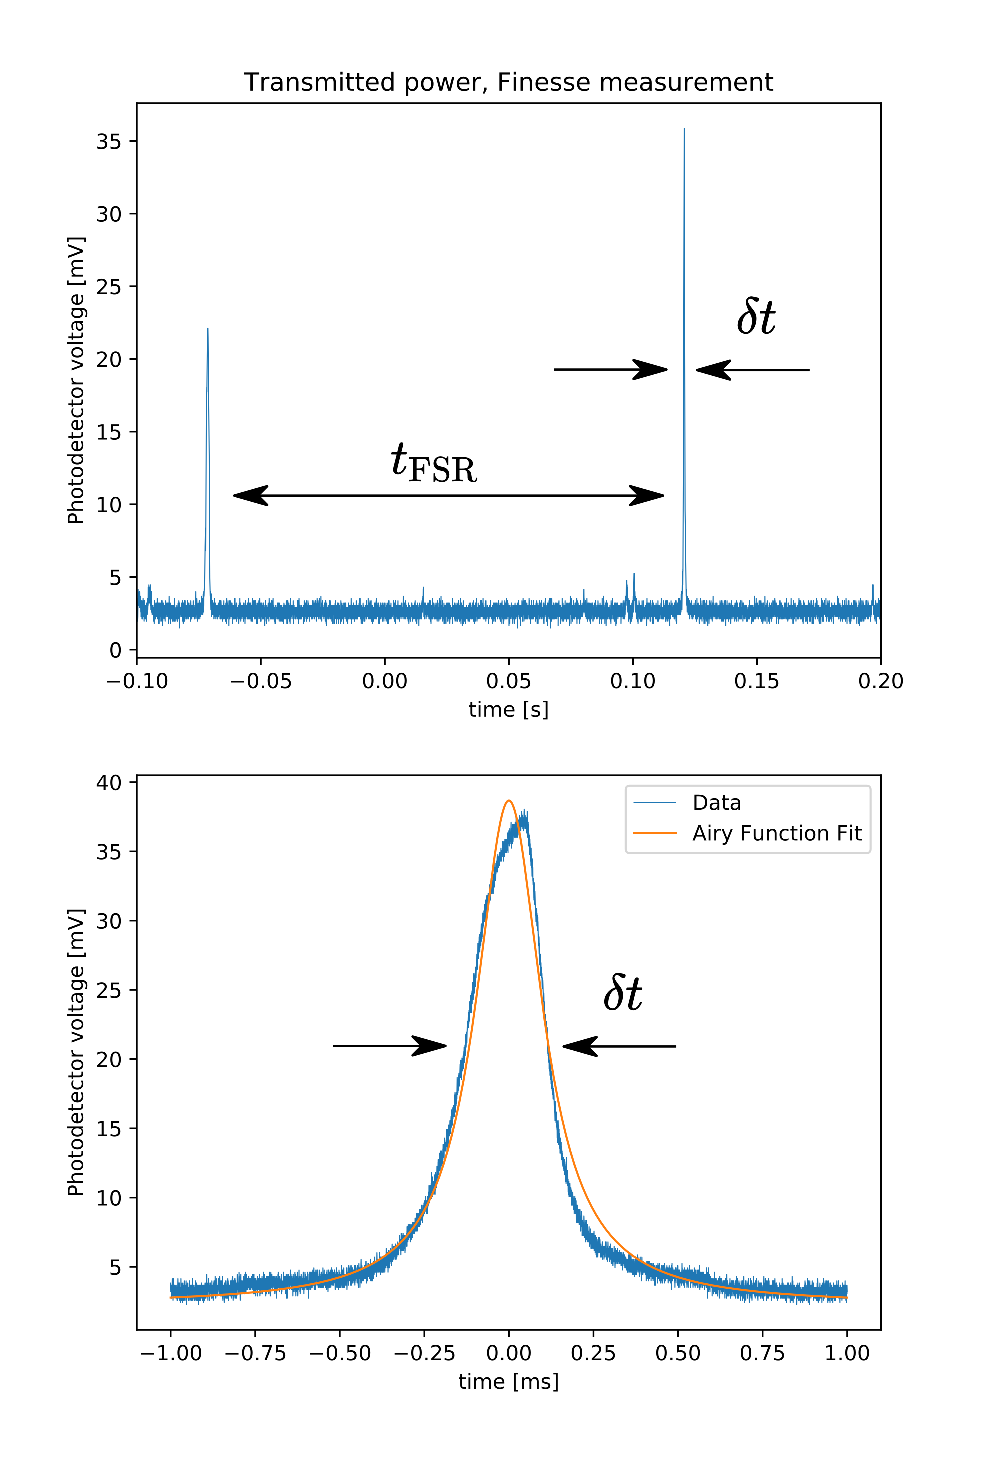
\includegraphics[width=0.9\linewidth]{images/FSRfinesse.eps}
	\caption{Finesse measurement by monitoring the transmitted power during a piezo scan of the cavity. Top: scan of a FSR of the cavity ($\delta L > 1030$\,nm), the two peaks correspond to $HG_{00}$ modes resonating inside the cavity. Bottom: scan of a single transmission peak, its width corresponds to the cavity linewidth. The deformation on the peak is due to noise on the scanning piezo.}
	\label{fig:FSRfinesse}
\end{figure}
The resonator Finesse, defined in eq. \ref{eq:finesse}, depends on the cavity losses and can be directly measured by measuring the cavity linewidth and the Free Spectral Range of the cavity. We recall that the power transmitted by the power depends on the detuning $\delta = 2\pi (\nu-\nu_0)L/c$ via eq \ref{eq:power}, so to find the cavity linewidth we can scan the cavity length using the piezo. In Fig \ref{fig:FSRfinesse} we see the transmitted power during a scan, the distance between two peaks corresponds to a change in cavity length of $\lambda = 1030$\,nm. The Finesse can be obtained by dividing the temporal interval between two peaks by the temporal FWHM of a peak. The peak shape must be optimized: if the scanning frequency is too low the piezo is subject to disturbances and noises that deform the peak shape, if it is too high the cavity might not reach the internal maximum power due to its higher characteristic time. The peak shape is then fitted with a Airy function (Fig \ref{fig:FSRfinesse}) to get the cavity linewidth, the result for the blue cavity is:
\begin{align}
	\mathrm{Finesse} = \frac{\nu_{\mathrm{FSR}}}{\delta\nu} =\frac{t_{\mathrm{FSR}}}{\delta t} = \frac{0.1922\,s}{(2.55\pm 0.10)\times 10^{-4}\,s} = 752 \pm 30
\end{align}
Where the error on the measurement is taken to be the difference in FWHM between the acquired data and the Airy function fit. 
The Finesse for the red cavity is instead measured to be $F = 406\pm25$.
\subsection{Power Spectral Density Noise measurement}

\begin{figure}
	\centering
	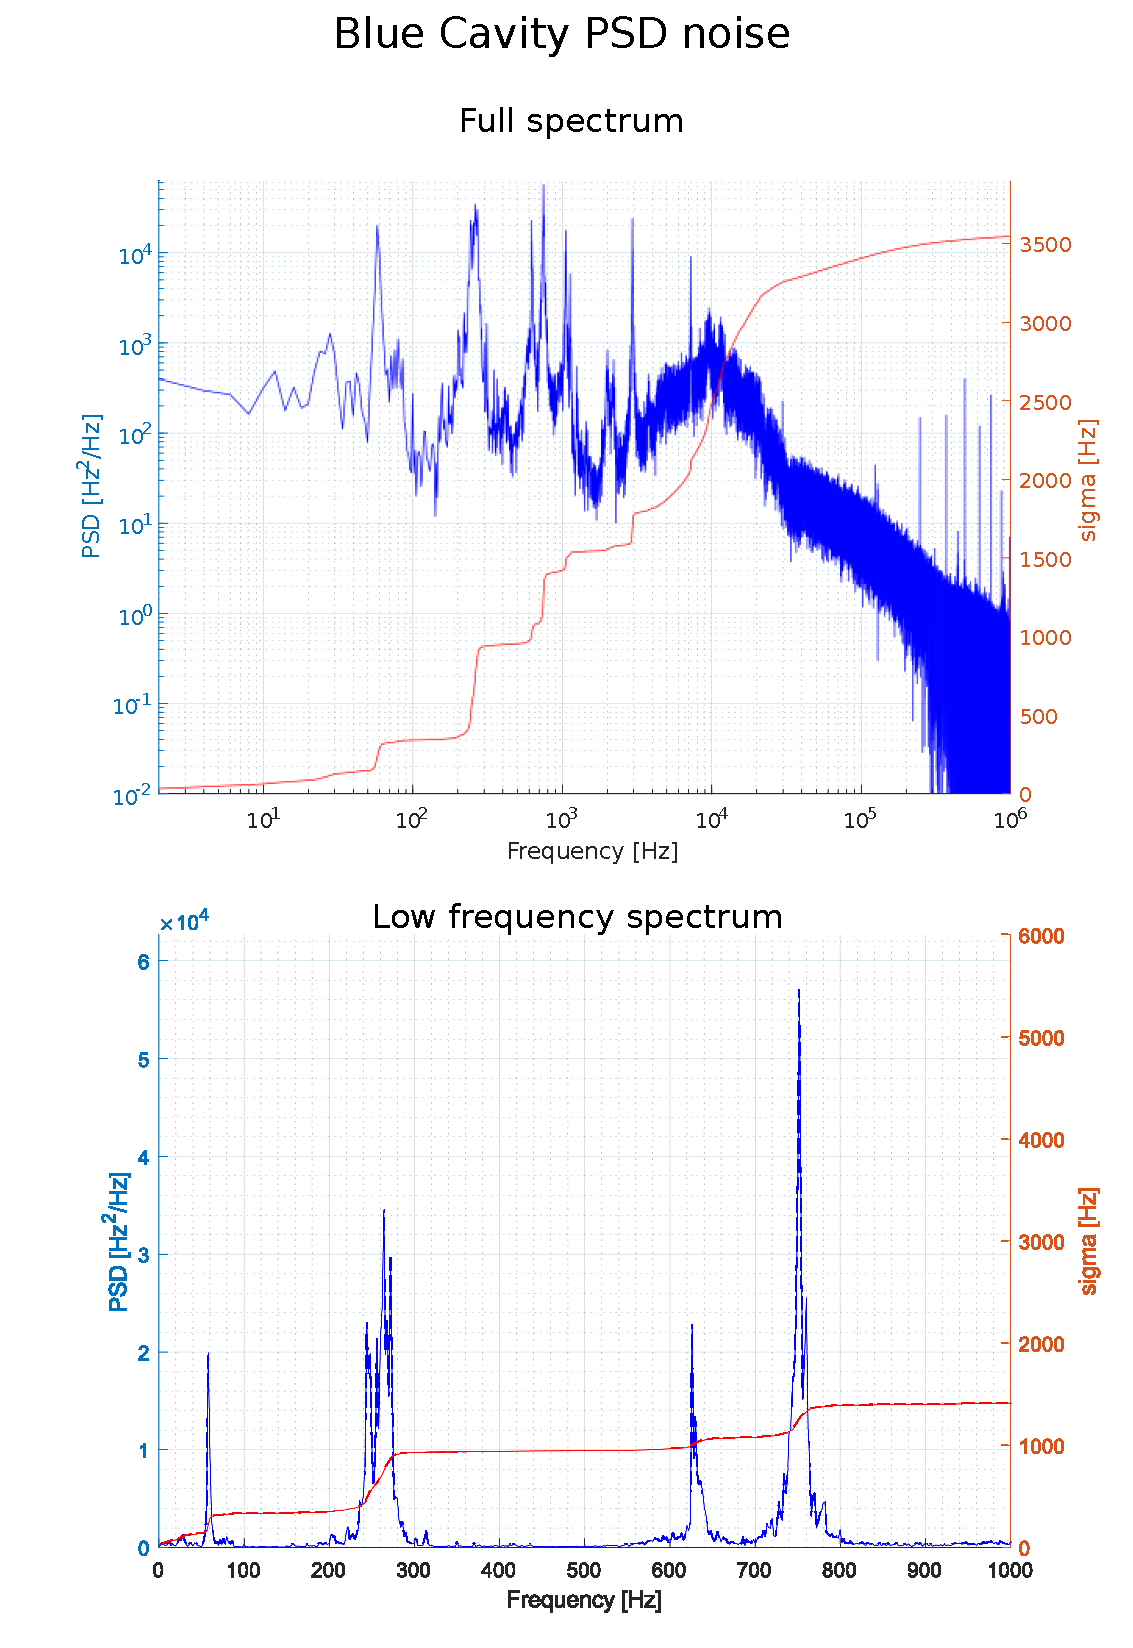
\includegraphics[width=0.9\linewidth]{images/PSD.eps}
	\caption{Power Spectral Density of the frequency noise between the blue cavity and the laser source. Top: full spectrum of the PSD, the broad peak at 10000\,Hz is due to the PDH system auto-oscillations. Bottom: low frequency spectrum of the PSD, each peak corresponds to a different mechanical harmonic oscillator in the system, such as the mirror mountings.}
	\label{fig:PSD}
\end{figure}
\begin{figure}
	\centering
	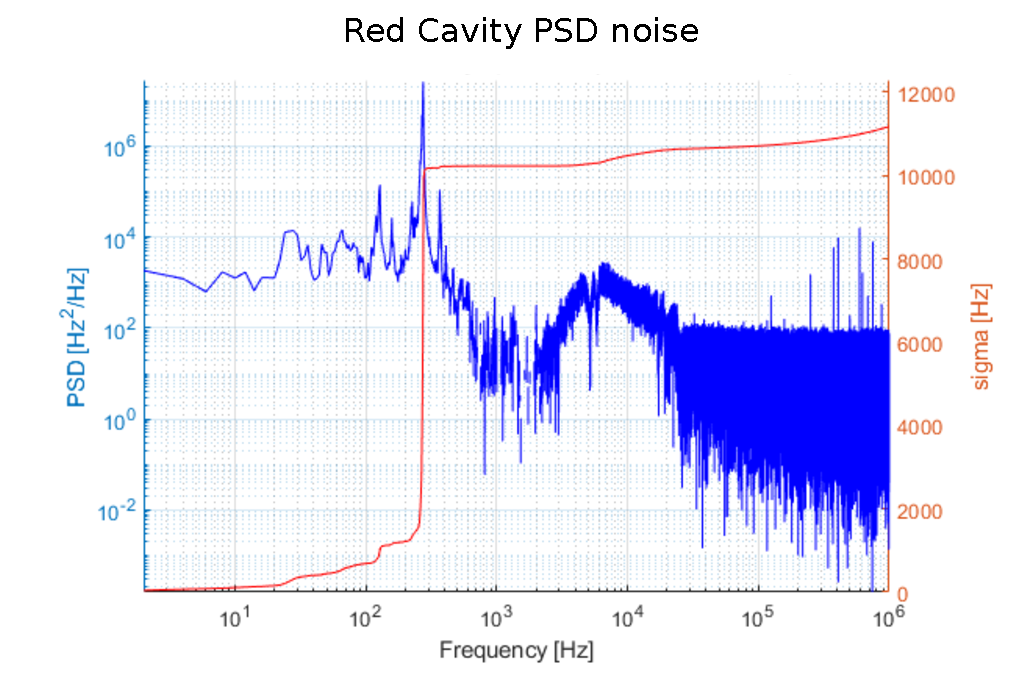
\includegraphics[width=0.9\linewidth]{images/rossabroad.eps}
	\caption{Power Spectral Density noise for the red cavity. The noise is much higher and primarly due to the low-frequency peak at 150\,Hz.}
	\label{fig:rossabroad}
\end{figure}

The cavity-laser system is subject to a variety of noise sources, from pump fluctuations in the oscillator to mechanical vibrations of the mirrors. These effects contribute to the cavity-laser detuning and are taken care by the stabilization system. To quantify this noise and describe it in the spectral domain a Power Spectral Density (PSD) noise measurement can be made. The PSD of a signal $x(t)$ is defined as
\begin{align}
	S(f) = \lim_{T\rightarrow\infty}\mathrm{E}\left[|\tilde x(f)|^2\right]
\end{align}
where E denotes the expected value and $\tilde x(f)$ is the truncated Fourier transform of $x(t)$:
\begin{align}
	\tilde x(f) = \frac{1}{\sqrt{T}} \int_{0}^{T}x(t) e^{-i2\pi ft} dt
\end{align}
Another equivalent definition is the Fourier transform of the autocorrelation function of the signal:
\begin{align}
	S(f) = \int_{-\infty}^{\infty} R(\tau) e^{-i2\pi\tau f} d\tau
\end{align}

We are interested in the frequency noise between the stabilized cavity and the laser source, since the PDH system works by translating a frequency noise difference in an asymmetric signal we can use the error signal generated by the discriminator to monitor the frequency noise and calculate its PSD.

The experimental procedure consists in the following steps:
\begin{enumerate}
	\item The cavity is stabilized as described earlier in the chapter, the stabilization parameters are optimized looking at the integrated noise on the oscilloscope.
	\item The error signal coming out of the mixer is sent to the oscilloscope and the signal is acquired on a 0.5\,s temporal window.
	\item The trace of the oscilloscope is acquired ten times while the cavity remains stabilized.
	\item To acquire the background signal the cavity is disrupted by blocking the ray inside it. The background signal is also acquired ten times.
	\item To obtain the frequency/voltage conversion factor ($k$) of the system the error signal is analyzed: we know the two sidebands are separated by 7\,MHz and from this the linear coefficient of the ``linear zone'' can be inferred.
	\item The data is analyzed by taking the PSD of each measurement, averaging them and subtracting the average PSD background.
\end{enumerate}

Results for the blue cavity are shown in Fig \ref{fig:PSD}, noise at low-frequencies is due mainly to mechanical vibrations while electronic noise, such as auto-oscillations of the stabilization system, is at high-frequencies. The integrated noise $\sigma$ corresponds to the $\sigma_{\mathrm{RMS}}$ of the error signal in the time domain. For the power inside the cavity to remain stable, this integrated noise must be much less than the cavity linewidth, in our case:
\begin{align}
	\frac{\sigma}{\delta\nu} = \frac{3500\,\mathrm{Hz}}{130000\,\mathrm{Hz}} \approx 0.027 \ll 1
\end{align}
Note that if we increase the cavity Finesse the integrated noise must be kept smaller to ensure good cavity stabilization, for this reason the PSD noise is used as a benchmark in the R\&D system: most upgrades (such as better and lower mountings and the breadboard) are finalized to reduce the cavity noise.

\subsection{Spatial and spectral coupling}

As noted before, good spatial and spectral coupling between the cavity fundamental mode and the outside laser mode must be achieved to ensure maximum power is reached inside the cavity. Spatial coupling can be optimized acting on the laser beam with a telescopic system and mirrors, ensuring its transverse profile matches that of the cavity fundamental mode (i.e. the overlap integral must be maximized). Spectral coupling is affected mainly by two factors: the laser source Carrier-Envelope-Offset and the mirror dispersion, the former can be controlled acting on the source with a stabilization system (not currently present in our setup) while the latter depends only on the nature of the cavity mirrors. In both cases by reducing the spectral width of the pulse incident on the cavity the spectral coupling can be increased.

\subsubsection{Spatial coupling}
\begin{figure}
	\centering
	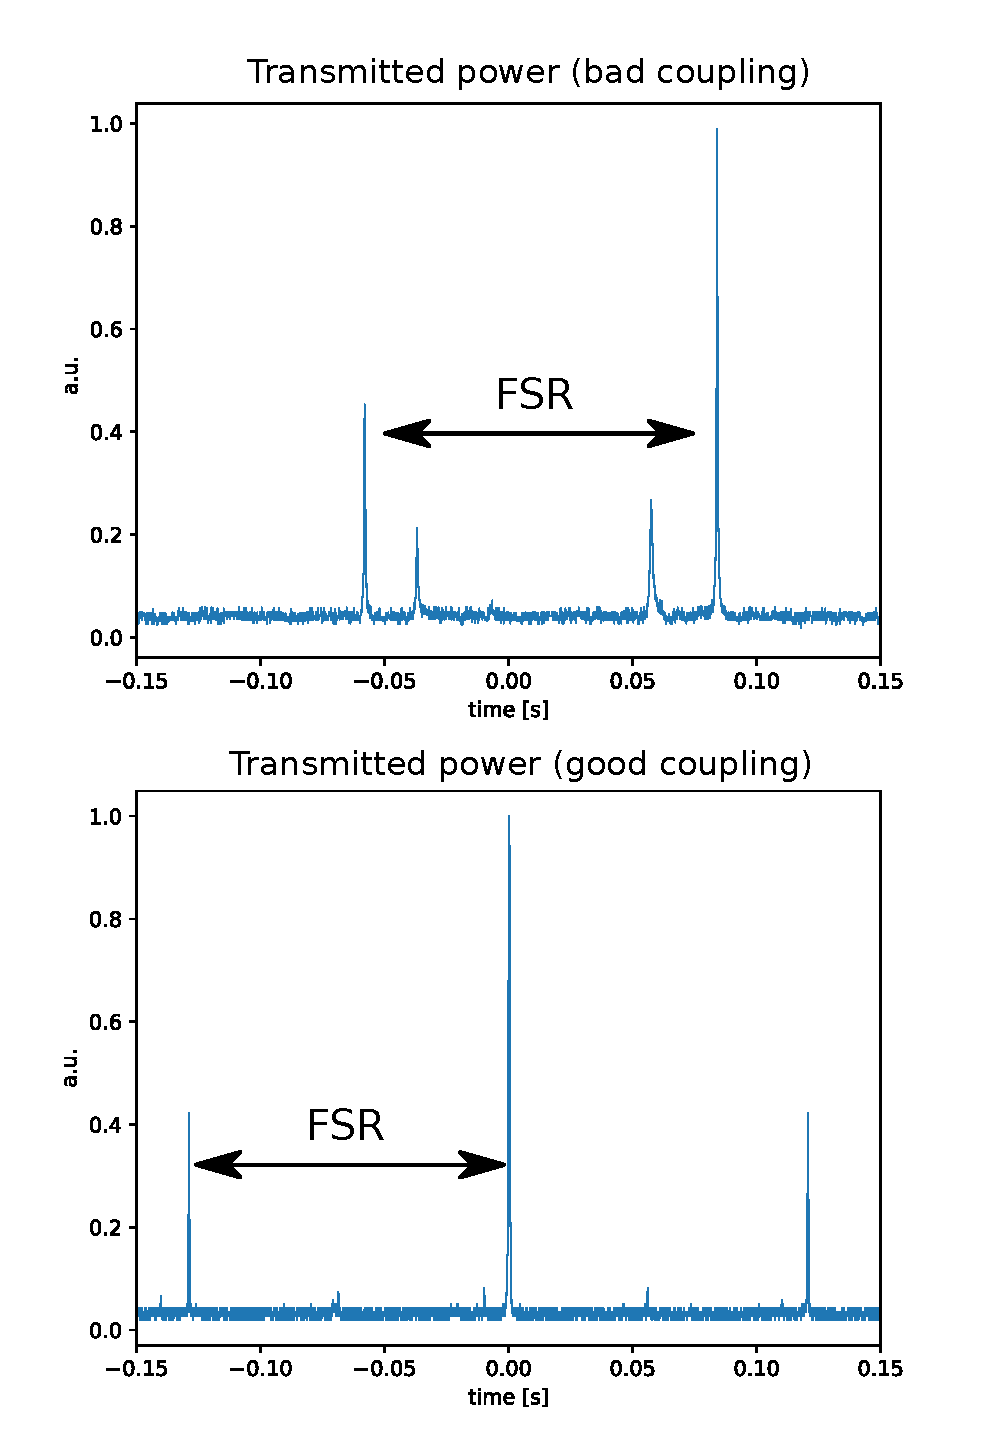
\includegraphics[width=0.9\linewidth]{images/goodspa.eps}
	\caption{Transmitted power in the cases of bad (top) and good (bottom) spatial coupling. When the spatial coupling is good only $HG_{00}$ modes resonate in the cavity (those separated by a FSR), when it is bad additional modes (usually first or second order modes) can resonate and other transmission peaks can be seen.}
	\label{fig:goodspa}
\end{figure}

The spatial coupling is quantified by the normalized overlap integral
\begin{align}
\frac{P_\mathrm{coupled}}{P_\mathrm{ext}} = \frac{	\left|\bra{\phi_\mathrm{ext}}\ket{\phi_{00}}\right|^2} {\bra{\phi_\mathrm{ext}}\ket{\phi_\mathrm{ext}}}
\end{align}
where $P_\mathrm{coupled}$ is the power coupled inside the cavity, $P_\mathrm{ext}$  is the total power incident on the cavity, $\ket{\phi_\mathrm{ext}}$ is the external laser mode and $\ket{\phi_{nm}}$ are the normalized cavity Hermite-Gauss modes. Since the Hermite-Gauss modes form a complete system and are orthogonal to each other we can write
\begin{align}
	\frac{P_\mathrm{coupled}}{P_\mathrm{ext}} = \frac{	\left|\bra{\phi_\mathrm{ext}}\ket{\phi_{00}}\right|^2} {\sum_{nm}\left|\bra{\phi_\mathrm{ext}}\ket{\phi_{nm}}\right|^2}
\end{align}

The power inside the cavity $P_\mathrm{in}$ (and the transmitted power) is directly proportional to the power coupled
\begin{align}
	P_\mathrm{in} \propto P_\mathrm{coupled} \propto \left|\bra{\phi_\mathrm{ext}}\ket{\phi_{00}}\right|^2
\end{align}
This means that by measuring the power transmitted by the cavity when each mode $\ket{\phi_{nm}}$ oscillates we can calculate the spatial coupling with the fundamental mode
\begin{align}
		\frac{P_\mathrm{coupled}}{P_\mathrm{ext}} = \frac{P_{00}}{\sum_{nm} P_{nm}}
\end{align}
where $P_{nm}$ is the power transmitted by the cavity when the mode $HG_{nm}$ is resonating.

To measure the transmitted power for each mode we scan the cavity with the piezo, the scanning time must be compatible with the characteristic cavity time to ensure maximum power is reached inside the cavity. The height of each transmission peak gives the transmitted power for the corresponding mode, we only need to measure the height of the peaks between two $HG_{00}$ modes since the pattern repeats itself every Free Spectral Range. In Fig \ref{fig:goodspa} we can see both cases of bad and good spatial coupling. The measurements indicate a spatial coupling of about 90\%.

\subsubsection{Spectral coupling}
\begin{figure}
	\centering
	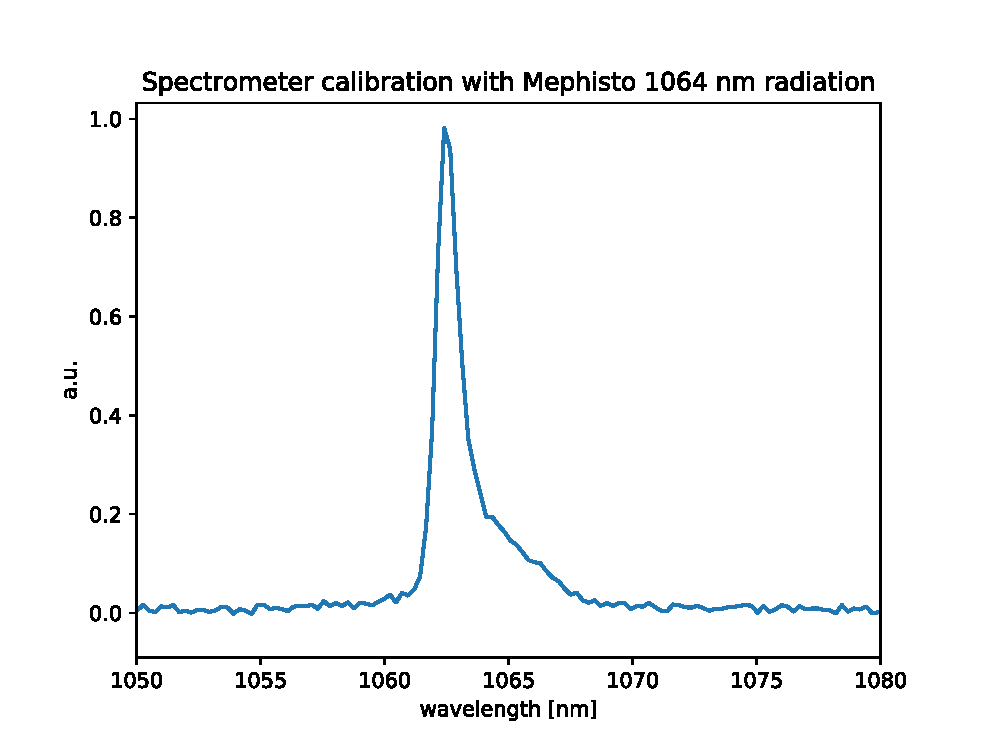
\includegraphics[width=0.9\linewidth]{images/mephisto.eps}
	\caption{Thorlabs CCD spectrometer calibration. The incident light is produced by a ultra-narrow bandwidth 1064\,nm CW laser. The FWHM, taken as instrument resolution, is $\delta\lambda = 1.2$\,nm. The broadening at the base is due to the multi-mode fiber propagation.}
	\label{fig:mephisto}
\end{figure}

To obtain the spectral coupling we can measure the spectrum of the radiation incident on the cavity and compare it with that of the transmitted radiation. For the measurement we used a CCD spectrometer from Thorlabs, the beam is sent to the spectrometer through an optical fiber. Good coupling with the fiber must be achieved in order to not alter the measured spectrum by pumping lateral modes of the multi-mode fiber. For this we used the fiber coupler shown in Fig \ref{fig:coupler}, which includes a converging lens.

\begin{figure}
	\centering
	\includegraphics[width=0.8\linewidth]{images/foto/coupler.jpg}
	\caption{The fiber coupler used for the measuring of the laser beam spectra, two such couplers has been used: one before the cavity and one after. At the center there is a converging lens, while the fiber is attached on the back, the regulation is done through two screws.}
	\label{fig:coupler}
\end{figure}

We first estimated the instrument spectral resolution by measuring the spectrum produced by a CW ultra-narrow linewidth laser (the Mephisto ND:YAG laser), the spectrometer response is shown in Fig \ref{fig:mephisto}, this response can be used to deconvolute the measurements to increase precision. It is worth to note that the response has been measured at 1064\,nm while the other measurements occur at 1030\,nm, where the instrument response could be different. From this we get a resolution of about $\delta \lambda =1.2$\,nm.

The procedure to acquire the radiation spectra consists in the following steps:
\begin{enumerate}
	\item The laser beam power is measured outside the cavity with a photodiode.
	\item The beam is coupled with a fiber coupler, the coupling is optimized until 85-90\% of the power is transmitted through the fiber.
	\item The fiber is connected to the spectrometer, the power must be reduced using optical filters not to saturate or damage the instrument.
	\item The input spectrum is acquired.
	\item The cavity is stabilized, and the transmitted beam is coupled in the fiber, again optimizing the power coupling.
	\item The output spectrum is acquired.
	\item The input and output spectrum are renormalized in intensity and their integrated profile compared to calculate the spectral efficiency.
\end{enumerate}

The first measurement has been done on the blue cavity with Finesse 750 (as shown earlier the coupling can depend on the Finesse).
The results, shown in Fig \ref{fig:6nm}, demonstrate that our instrument has a resolution too small to differentiate between the input and output spectrum, as they appear to be about the same width in both cases (6\,nm input and 10\,nm input).
Another factor that may obscure the difference is that the coupling with the fiber may be different between the two measures. Within the resolution of our instrument, we can say that the spectral coupling efficiency is very high ($>85\%$). According to the results of the next section regarding mirror reflectivities, the coupling efficiency is even higher.

\begin{figure}
	\centering
	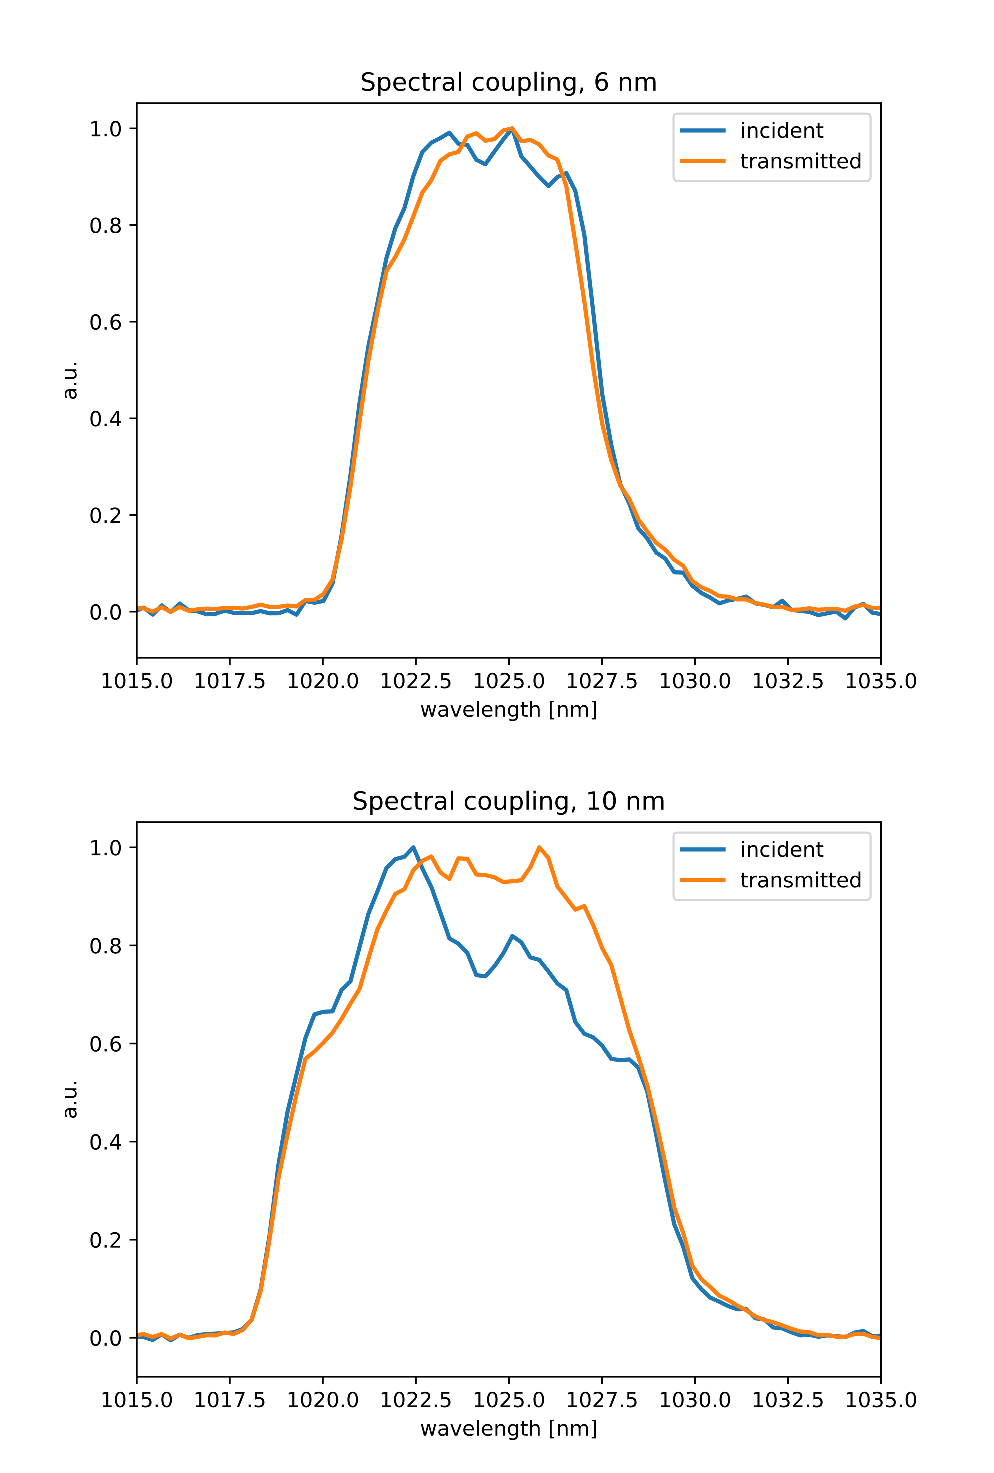
\includegraphics[width=0.9\linewidth]{images/6nm.eps}
	\caption{Spectra for the radiation incident on the cavity and transmitted by the cavity. The difference is too small if confronted with the spectrometer resolution so the spectra appear similar.}
	\label{fig:6nm}
\end{figure}

To demonstrate that the experimental procedure is correct, we can change the $f_\mathrm{CEO}$ and verify that the spectral coupling changes with it (as shown earlier, Fig \ref{fig:couplingeta}). Note that we can't directly control the offset, but since it depends on the temperature of the lasing medium, we can change it by varying the laser diode current. In Fig \ref{fig:currents} we can see that the radiation spectrum at the output depends strongly on the diode current. In this case the coupling with the fiber remains the same, since the apparatus is the same for all measures, and the differences in the transmitted radiation spectra are more evident.

\begin{figure}
	\centering
	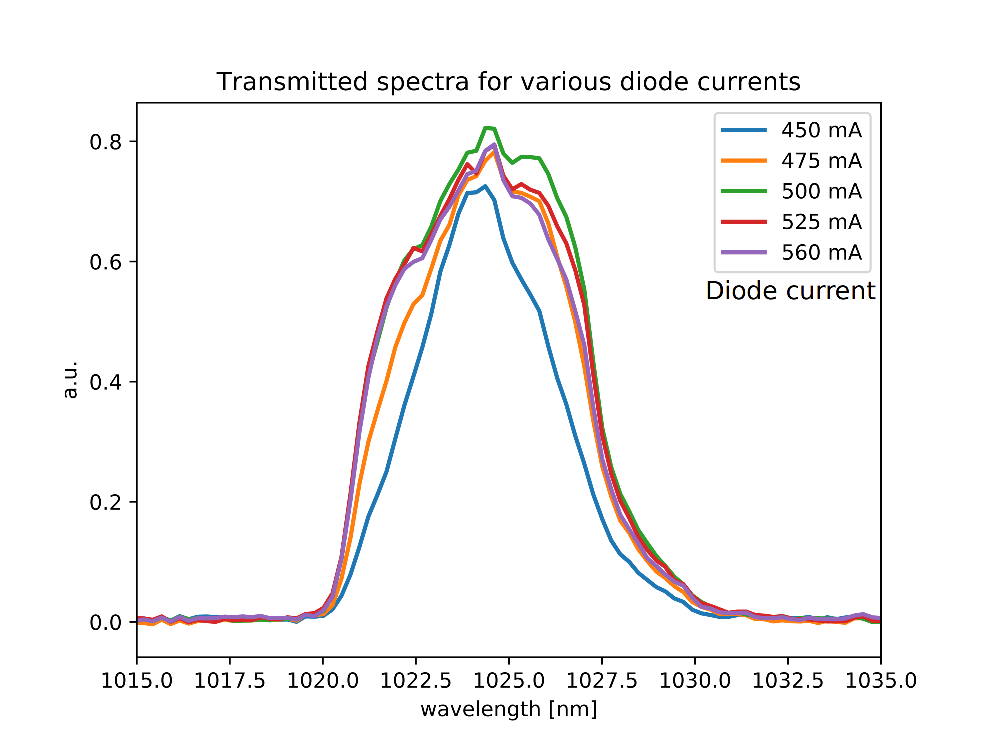
\includegraphics[width=0.9\linewidth]{images/currents.eps}
	\caption{Different transmitted spectra obtained by changing the Menlo laser diode current. The change in current translate to a change in temperature in the active medium, this changes the $f_\mathrm{CEO}$ and so the spectral coupling (see Fig \ref{fig:couplingeta}). In this case the best spectral coupling is obtained for 500\,mA.}
	\label{fig:currents}
\end{figure}

We then replaced the input coupler, going from 99.2\% reflectivity to about 99.8\% and increasing the cavity Finesse to about 3000.
We again measured the spectral coupling, changing the oscillator diode current. This time we were able to measure a spectral coupling efficiency of about 90\% for all cases, the improvement is probably due to better fiber coupling. The results are shown in Fig \ref{fig:accspe} and Tab \ref{tab:coup3000}. The differences between the measurement are due to a different value for the $f_\mathrm{CEO}$.

\begin{figure}
	\centering
	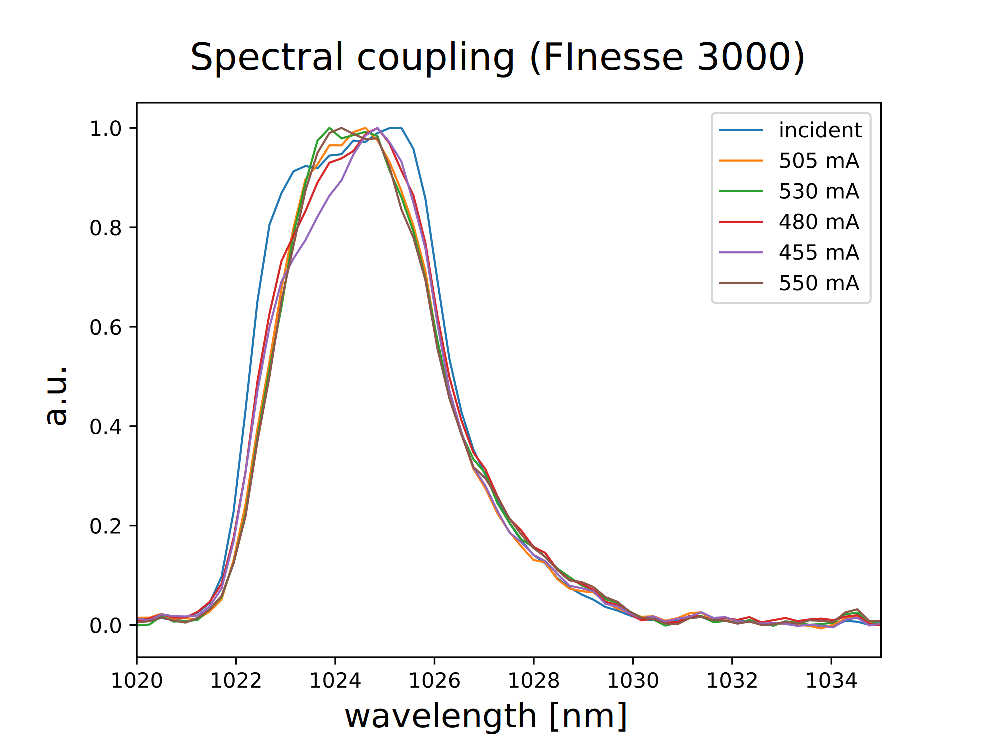
\includegraphics[width=0.9\linewidth]{images/accspe.eps}
	\caption{Different transmitted spectra for the Finesse 3000 cavity. In this case the best spectral coupling is obtained for 480\,mA.}
	\label{fig:accspe}
\end{figure}
\begin{table}
	\centering
	\begin{tabular}{|c|c|c|c|}
		\hline 
		current [mA]&spectral coupling & $P_\mathrm{ref}/P_\mathrm{in} $ & Mirrors reflectivity\\ 
		\hline 
		505	& $0.9\pm5$ & 0.62 & $0.99996 \pm0.00005$ \\ 
		\hline 
		530	& $0.91\pm5$ & 0.65 & $0.99998 \pm0.00005$\\ 
		\hline 
		550	& $0.91\pm5$ & 0.65 &$0.99998 \pm0.00005$ \\ 
		\hline
		480	& $0.96\pm5$ & 0.56 &$0.99983 \pm0.00005$ \\ 
		\hline
		505	& $0.91\pm5$ & 0.56 &$0.99990 \pm0.00005$ \\ 
		\hline
	\end{tabular}
	\caption{Spectral coupling for the blue cavity at Finesse 3000. The reflected power is used to calculate mirror reflectivities. The error on the spectral coupling is given by the instrument resolution (Fig \ref{fig:mephisto}), and that on the reflectivity by error propagation. The measurement at 480\,mA gives an efficiency higher than the others that results in a lower reflectivity. The other measurements are compatible with a reflectivity of 99.995\% for mirrors B C and D.}
	\label{tab:coup3000}
\end{table}

\subsubsection{Mirror reflectivities}

If we consider spatial and spectral coupling efficiencies $\eta_1$ and $\eta_2$ in calculating the power reflected by the cavity when in resonance (eq. \ref{eq:ref}), we get
\begin{align}
\frac{P_\mathrm{ref}}{P_\mathrm{in}} = \left[ \frac{\sqrt{\eta_1\eta_2}(1-R_1)\sqrt{R_2R_3R_4}}{1-\sqrt{R_1R_2R_3R_4}}-\sqrt{R_1}  \right]^2
\end{align}
From the equation we can see that by measuring the reflected power when the cavity is stabilized, and by knowing the efficiencies, we can estimate the total mirrors reflectivity $R_2R_3R_4$. For this purpose, we consider the reflectivity of the input coupler $R_1$ to be that indicated by the supplier (Layertec): $99.25\%$ (this is in accordance with the Finesse measurement). The previous Finesse measurement gives a minimum reflectivity of about 99.98\% for each mirror\footnote{The Finesse provides only a minimum figure because other losses contribute to the Finesse measured value.}.

To measure the reflectivities we then proceed as follows:
\begin{enumerate}
	\item The input radiation spectrum is acquired, following the steps described earlier.
	\item The reflected power (out of resonance) is measured.
	\item The spatial coupling efficiency is calculated looking at the transmission peaks.
	\item The cavity is stabilized.
	\item The transmitted radiation spectra is acquired.
	\item The reflected power (in resonance) is measured.
	\item The spectra are confronted to estimate the spectral coupling efficiency.
\end{enumerate}

The measurement of the spectral coupling efficiency $\eta_2$ is not precise, but using the other data we can plot (Fig \ref{fig:reflectivities}) the mirror reflectivities $R$ ($R=R_2=R_3=R_4$) as a function of $\eta_2$. From the plot we can see that $\eta_2$ must be over 92\%. The two measurements are compatible with a mirror reflectivity around 99.995\% estimating $\eta_2$ at 95\%.

The calculation has also been made with the results obtained using the coupler with 99.8\% reflectivity, but since we weren't able to accurately measure the Finesse of the cavity we cannot yet trust the nominal reflectivity value (new methods for measuring the Finesse are being developed in our laboratory). The results assuming the mirror A nominal reflectivity are in Tab \ref{tab:coup3000}.
\begin{table}
	\centering
	\begin{tabular}{|c|c|c|}
		\hline 
		data  &$P_\mathrm{ref}/P_\mathrm{in}$ &$\eta_1$ \\ 
		\hline 
		6\,nm	& 0.59 & 89\% \\ 
		\hline 
		10\,nm	& 0.67 & 90\% \\ 
		\hline 
		
	\end{tabular}
	\caption{Data points for the mirror reflectivity measurements. $\eta_1$ is the spatial coupling efficiency.}
	\label{tab:ref}
\end{table}

\begin{figure}
	\centering
	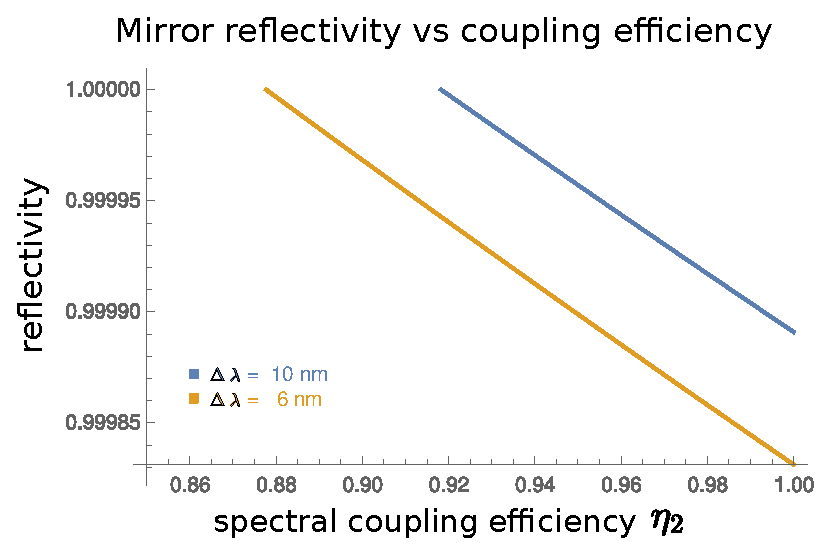
\includegraphics[width=0.9\linewidth]{images/reflectivities.eps}
	\caption{Mirror reflectivity for different values of the spectral coupling efficiency. The two colors indicate two different measurements (data in Tab \ref{tab:ref}). If we estimate $\eta_2$ to be about 95\% the measurements are compatible with a mirror reflectivity of 99.995\%.}
	\label{fig:reflectivities}
\end{figure}

\subsection{Compensation method}

As explained earlier, the compensation method will be used to address the issue of thermal deformation of the mirrors at high power. The measurement is available thanks to the piezo-driven linear stages represented in Fig \ref{fig:smaract}.

The sleds can move in two different ways, named scan mode and step mode. When in scan mode, the voltage on the piezo is directly controlled (from 0\,V to up to 100\,V). In step mode, the piezo is subjected to an alternate voltage and undergoes several cycles of stretching and contracting, resulting in an overall movement in the specified direction\footnote{This technology is called ``Stick-Slip Drive'', further details can be found at \url{https://www.smaract.com/technology-introduction-and-options}.}. While the sled can move macroscopically in step mode, the distance covered in scan mode is given only by the piezo crystal properties and amounts to $\approx 0.5\,\mu$m.

Two sleds are needed to change the distance between the curved mirrors and to restore the cavity length. An application written in LabView has been developed to move both the sleds at the same time. We have verified that movement in step mode is not possible, as the stabilization system is not able to correct for the sudden changes in cavity length, while this doesn't happen for a movement in scan mode. To achieve the distances required by the correction (that are on the order of a millimeter, Fig \ref{fig:compensation}) a new kind of long-distance moving piezo driven mirror mounting is been developed and characterized.

The experimental procedure consists in:
\begin{enumerate}
	\item placing the sled in the correct position for the movement (since they must go in opposite ways, one can be placed at 0\,V while the other at 100\,V)
	\item locking the cavity using the stabilization system
	\item moving the sleds simultaneously 
\end{enumerate}
\begin{sidewaysfigure}
	\centering
	\includegraphics[width=0.9\linewidth]{images/smaractmove.pdf}
	\caption{Moving the piezo-driven sleds in the stabilized cavity. The first two rows show the effect of moving a single sled, the PDH piezo corrects the change in cavity length and maintains the transmitted beam stable. The last row show the effect of moving both at the same time: tha cavity length is unchanged.}
	\label{fig:smaractmove}
\end{sidewaysfigure}

The transmitted beam has been monitored to ensure that the stabilization system is fast enough to correct the movements in real time, also the voltage on the piezo used by the stabilization system has been monitored to measure the change in cavity length. The results, shown in Fig \ref{fig:smaractmove}, show that when moving both the sleds the cavity length is unaffected (voltage on PDH piezo is constant), and the transmitted power is unchanged (and so the cavity internal power). By monitoring the voltage on the PDH piezo we can measure that by moving only one sled we change the cavity length of about $430\,$nm, since we know a wavelength ($\lambda = 1030\,$nm) corresponds to a change of about 7\,V on the PDH piezo.

\subsection{Cavity waist movement}

As demonstrated in the theoretical chapter, by inclining the curved mirrors we can move the cavity waist between them, this technique will be used in BriXS to change the cavity that interacts with the electron beam, enabling the dual color mode. To achieve the movement we used piezo-driven tilting mirrors that use the same ``Stick-Slip Drive technology'' as the sleds, again in scan mode.

\subsubsection{Mirror tilting measurement}
\begin{figure}
	\centering
	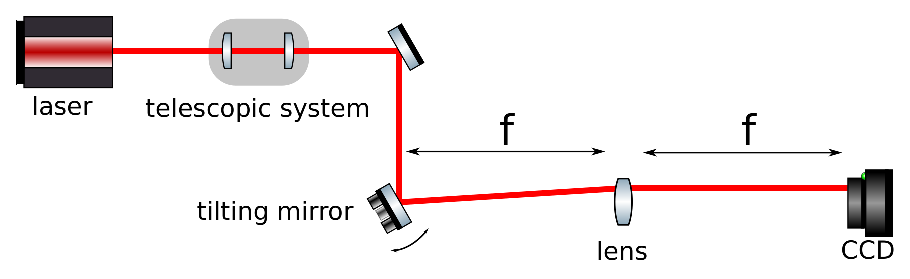
\includegraphics[width=0.9\linewidth]{images/tiltingme.eps}
	\caption{The apparatus used to measure the voltage-angle relation for the tilting mirrors. The telescopic system is used to collimate the beam. The focal length $f$ of the lens is 500\,mm.}
	\label{fig:tiltingme}
\end{figure}
\begin{figure}
	\centering
	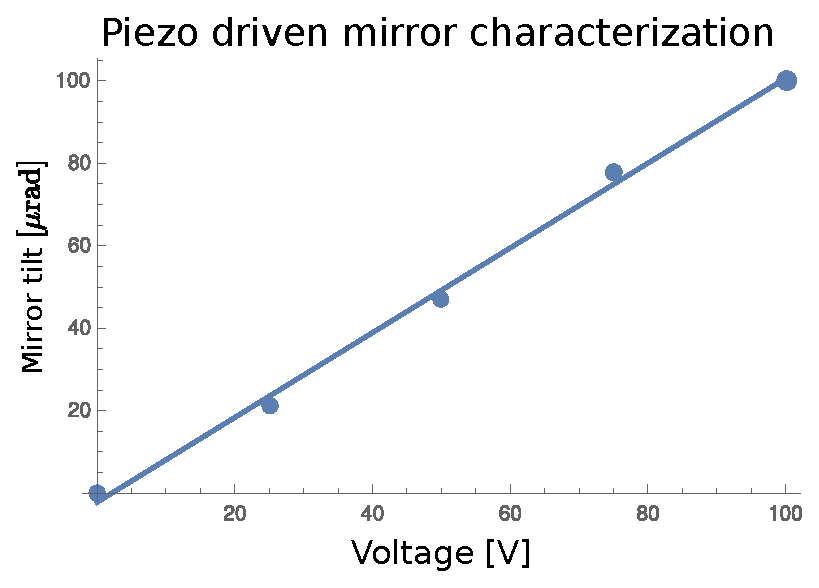
\includegraphics[width=0.8\linewidth]{images/mirrortilt.eps}
	\caption{Voltage-angle relation for the tilting mirrors. The relation is linear, with a max movement of $100\,\mu$rad.}
	\label{fig:mirrortilt}
\end{figure}

To characterize the tilting mirror mountings (i.e. to find the voltage-angle relation) we shine a laser at the mirror and monitor the movement of the beam with a CCD camera, after passing through a lens. The system is shown in Fig \ref{fig:tiltingme}. To relate the movement on the camera sensor with the angular movement we write the ABCD matrix for the system starting on the mirror surface, it is composed by a free space propagation of length $f$, a lens of focal length $f$ and another free space propagation:
\begin{align}
\begin{bmatrix}
1 & f \\
0 & 1 \\
\end{bmatrix}
\begin{bmatrix}
1 & 0 \\
-1/f & 1 \\
\end{bmatrix}
	\begin{bmatrix}
	1 & f \\
	0 & 1 \\
	\end{bmatrix}
	\begin{bmatrix}
	0 \\
	\theta  \\
	\end{bmatrix}
	=
	\begin{bmatrix}
	f\theta \\
	0  \\
	\end{bmatrix}
\end{align}

where $\theta$ is the initial ray inclination given by the tilting mirror. Note that if the ray has inclination $\theta$ that means that the mirror has moved by $\theta/2$.
The measurement gives a linear relation between voltage and angular tilt (Fig \ref{fig:mirrortilt}), with a maximum movement of 100\,$\mu$rad. According to the previous calculation that means that we can achieve a vertical shift of the waist of about 80\,$\mu$m. To achieve the movement required for BriXS (110\,$\mu$m) we are developing a new tilting mounting with a longer stroke. The new mountings will also be gimbal-like to avoid changing the cavity length during the movement.


\subsubsection{Focus movement measurement}

To directly observe the cavity waist during the movement we placed a high transmission plate inside the cavity at the focus location. A small part of the beam is reflected and can be used for an imaging of the focus. To find the waist location inside the cavity we observe the beam shape: since the cavity is astigmatic and near-confocal along the vertical direction its shape will be that of an horizontal ellipsoid near the focus, and that of a vertical ellipsoid away from it.

\begin{figure}
	\centering
	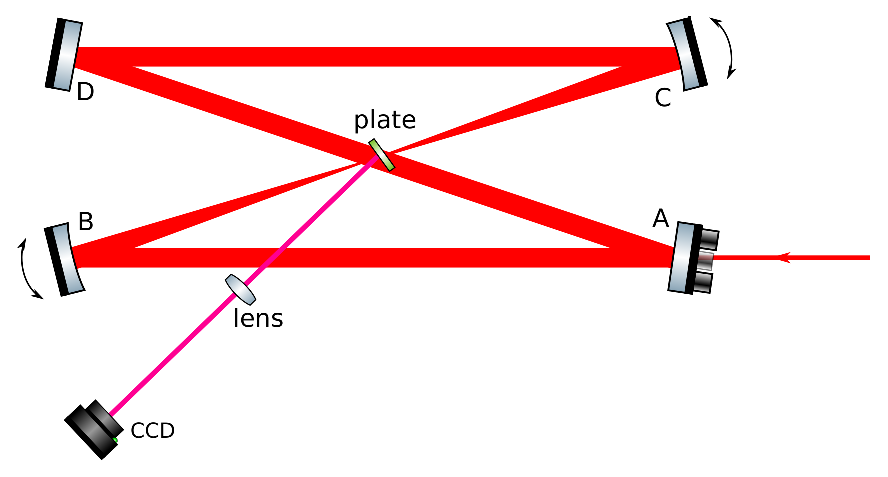
\includegraphics[width=0.8\linewidth]{images/focusima.eps}
	\caption{Apparatus for the imaging of the cavity waist.}
	\label{fig:focusima}
\end{figure}

After placing the imaging system, we can calculate the magnification factor by measuring the CCD-lens distance using
\begin{align}
	M = -\frac{q}{p} && \frac{1}{f} = \frac{1}{p} + \frac{1}{q}
\end{align}
where $p$ and $q$ are the distances of the waist and the camera from the lens, and $f$ its focal length. In our case
\begin{align*}
	p = 286\,\mathrm{mm} &&q = 315\,\mathrm{mm} &&f = 150\,\mathrm{mm} && M = -1.1
\end{align*}
Note that $M$ is negative so the image is inverted. The measured waist size $w$ is
\begin{align*}
	w_\mathrm{H} = 87\,\mu\mathrm{m} && w_\mathrm{V} = 61\,\mu\mathrm{m} 
\end{align*}

The procedure to measure the cavity waist movement consists in stabilizing the cavity, measuring the waist position using the image on the CCD camera, moving mirrors B and C at the same time and then repeating the position measurement.
During the movement we monitored the transmitted power and the PDH piezo voltage, to measure the shortening in cavity length.
In Fig \ref{fig:imagemov} and Fig \ref{fig:tilt} we see the images acquired during a movement and the relative data, the movement has been done applying a mirror tilt of 50\,$\mu$rad in a time of 55\,ms, resulting in a vertical shift of 36\,$\mu$m, in accordance with the predicted value of eq. \ref{fig:shiftfocus}. The transmitted power is unchanged before and after the movement, while during the movement it undergoes fluctuations. As indicated by the tension on the PDH piezo voltage, the cavity length changes by about $2\,\mu$m, corresponding to 14\,V.
\begin{figure}
	\centering
	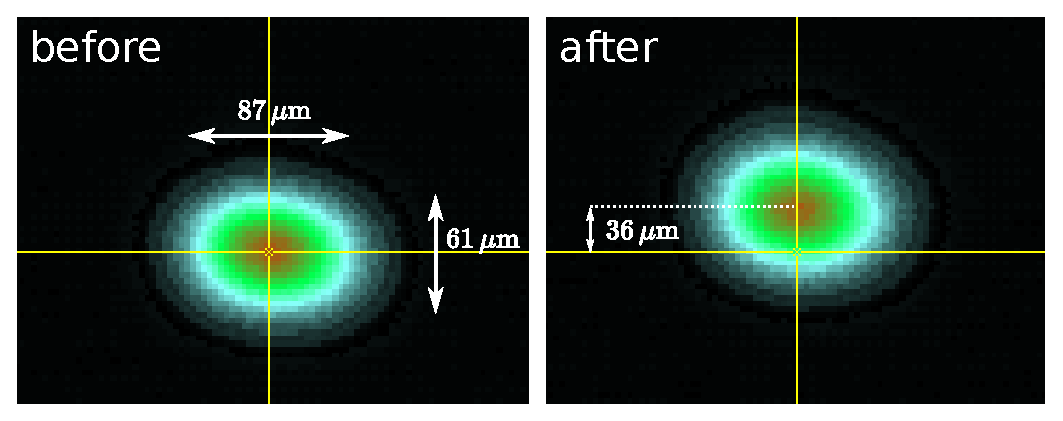
\includegraphics[width=1\linewidth]{images/imagemov.eps}
	\caption{Imaging of the cavity waist before and after the movement. To measure the beam radius $w$ and the shift the intensity profile has been fitted with a gaussian function.}
	\label{fig:imagemov}
\end{figure}
\begin{figure}
	\centering
	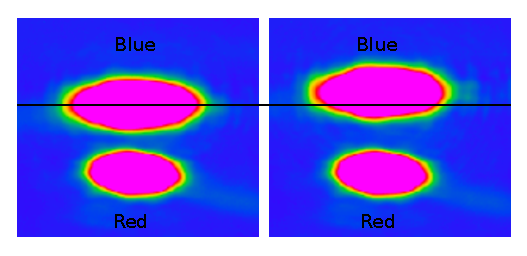
\includegraphics[width=1\linewidth]{images/doublefocus.eps}
	\caption{Waist movement while both cavities are stabilized.}
	\label{fig:doublefocus}
\end{figure}
\begin{figure}
	\centering
	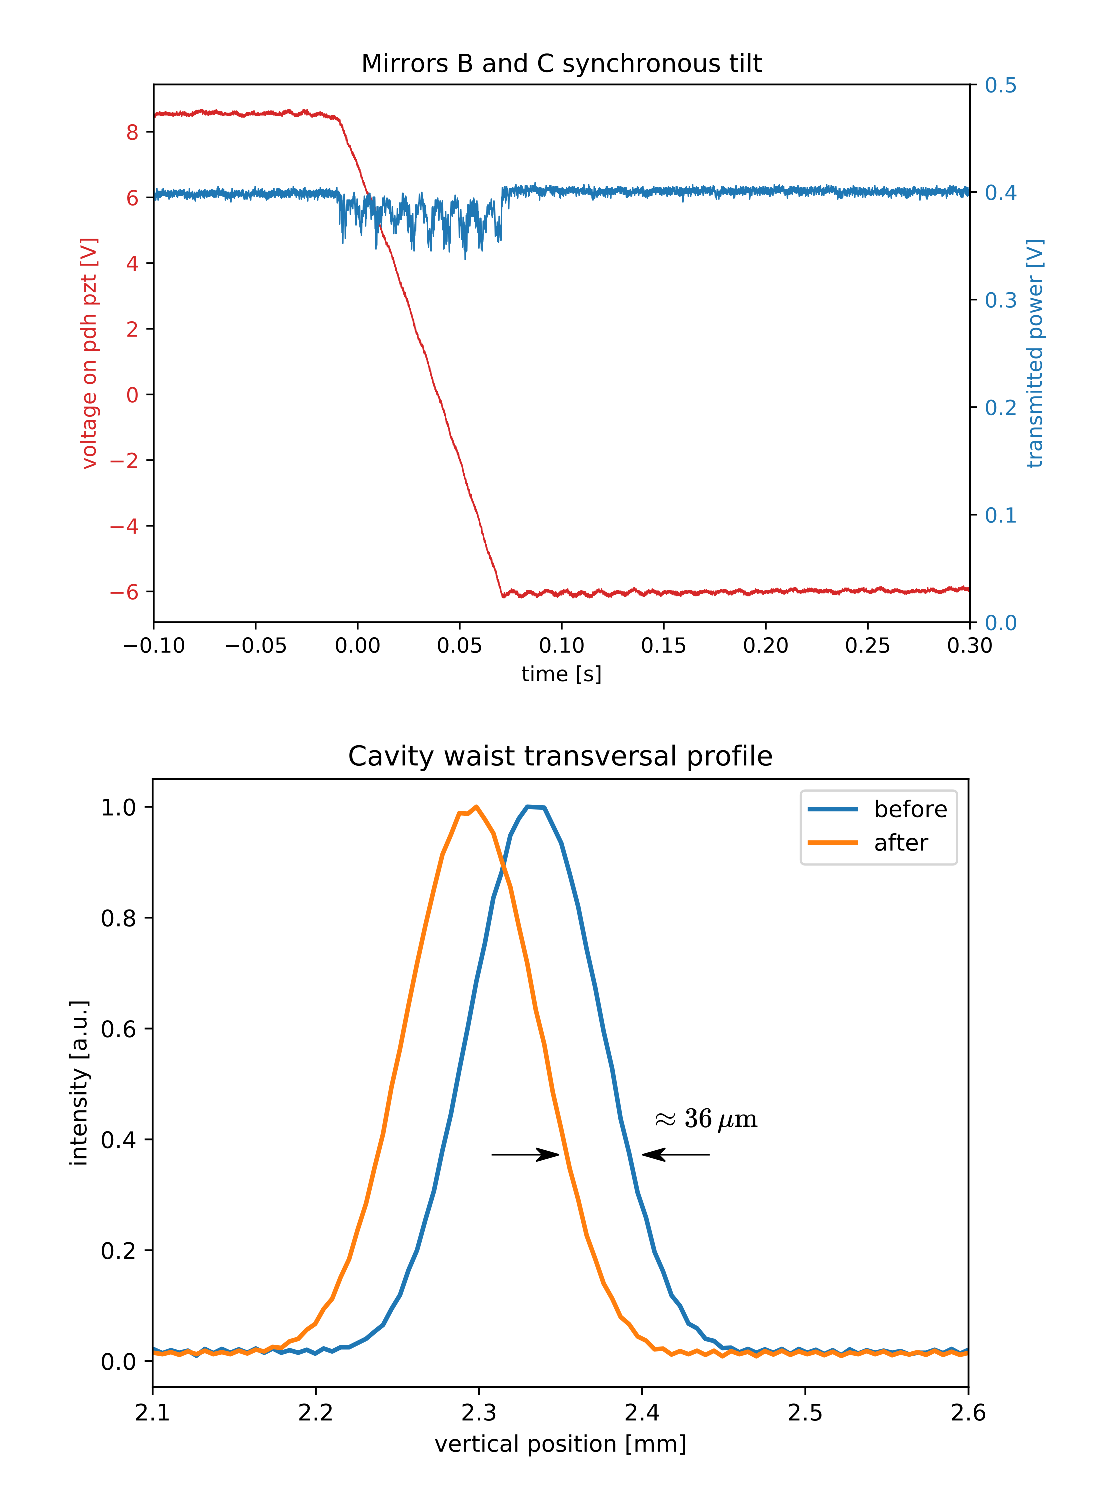
\includegraphics[width=0.9\linewidth]{images/tilt.eps}
	\caption{Top: transmitted power and PDH piezo voltage during the movement. Bottom: vertical intensity profile of the beam waist along the vertical direction, before and after the movement (not corrected with the imaging magnification factor $M$).}
	\label{fig:tilt}
\end{figure}

In Fig we can see the movement of one focus while both the red and blue cavity are stabilized, using the full tilting range of the mirrors the movement is about $80\,\mu\mathrm{rad}$. Only one cavity is currently equipped with the moving mirrors.



The measurement demonstrates the possibility of moving the laser beam of the two BriXS cavities in and out of the interaction point with the electrons, in a very short time ($\sim 100\,$ms) compatible with its medical applications.